\documentclass{beamer}
\usepackage{xeCJK}

\mode<presentation> {

\usetheme{Boadilla}
\usecolortheme{rose}

%\setbeamertemplate{footline} % To remove the footer line in all slides uncomment this line
%\setbeamertemplate{footline}[page number] % To replace the footer line in all slides with a simple slide count uncomment this line

%\setbeamertemplate{navigation symbols}{} % To remove the navigation symbols from the bottom of all slides uncomment this line
}

\usepackage{graphicx} % Allows including images
\usepackage{booktabs} % Allows the use of \toprule, \midrule and \bottomrule in tables

\title[答辩]{浅析居民消费异质性及其对经济增长路径的影响} % The short title appears at the bottom of every slide, the full title is only on the title page

\author{罗浩威} % Your name
\institute[] % Your institution as it will appear on the bottom of every slide, may be shorthand to save space
{
华中科技大学\\ % Your institution for the title page
\medskip
\textit{LoweetLo@outlook.com} % Your email address
}
\date{\today} % Date, can be changed to a custom date

\begin{document}

\begin{frame}
\titlepage % Print the title page as the first slide
\end{frame}

\begin{frame}
\frametitle{Overview} % Table of contents slide, comment this block out to remove it
\tableofcontents % Throughout your presentation, if you choose to use \section{} and \subsection{} commands, these will automatically be printed on this slide as an overview of your presentation
\end{frame}
%------------------------------------------------
\section{引言} % Sections can be created in order to organize your presentation into discrete blocks, all sections and subsections are automatically printed in the table of contents as an overview of the talk
%------------------------------------------------

%\subsection{Subsection Example} % A subsection can be created just before a set of slides with a common theme to further break down your presentation into chunks

\begin{frame}
\frametitle{引言}
\begin{itemize}
\item 中国经济崛起,房地产市场与金融市场不断改革开放后,居民财产得以迅速积累
\item 家庭财产结构及不同组成部分的特性将对消费产生重要的影响
\item 在新的全球环境下消费正逐渐成为经济增长的新动力
\item 我国长期以来居民消费水平与人均GDP之比不断下滑
\end{itemize}
\end{frame}

\begin{frame}
\frametitle{引言}
如何协调消费与储蓄、投资的关系,建立扩大消费需求的长效机制,释放中国居民强大的消费潜力成为了问题的关键,对居民消费行为的研究及对消费于经济增长路径所造成影响的分析将具有一定的重要性。
\end{frame}

\begin{frame}
\frametitle{引言}
\begin{itemize}
\item 传统的生命周期持久收入假说(Friedman,1957;Hall,1978)
\item BufferStock模型(Deaton 1991;Carroll 1997)
\item 异质性消费者理论(Campbell$\&$Mankiw,1989)
\item 后续实证(Chyi$\&$Huang,1997;Himarios,2000)
\item 异质性消费者理论对于国家财政政策与货币政策的影响(Gali et al,2005;Morita,2015;Natvik,2012)
\item 美国政府多次退税以刺激消费
\end{itemize}
\end{frame}

\begin{frame}
\frametitle{引言}
\begin{itemize}
\item 居民对于临时性收入冲击具有正的边际消费倾向(Misra$\&$Surico,2014;Johnson et al,2006;Shapir$\&$Slemrod,2003)
\item 以缺乏流动性资产、缺少信贷渠道来解释异质性消费(Zeldes,1989)
\item 从“有限理性”及信息不完全出发,解释“短视”消费为实际消费路径与最优化消费路径产生偏差的原因(Lettau$\&$Uhlig,1999;Blanchard,1985;Kotlikoff et al,1988)
\item 开创性地假定居民中存在一部分的HtM消费者(Kaplan$\&$Violante,2014)
\end{itemize}
\end{frame}

\begin{frame}
\frametitle{引言}
\begin{block}{Block 1}
HtM消费者假设目前存在的问题在于前人结合家庭金融调查数据并根据以净资产数额判断异质性消费者的方法发现净资产近乎于零、只得耗尽每期收入用于消费的消费者在人口中占比太小,不足以在数据中显现出上述的效果
\end{block}

\begin{block}{Block 2}
已有文献中的异质性消费者理论框架并不注重对家庭资产结构及不同资产流动性与收益加以探究
\end{block}

\begin{block}{Block 3}
已有文献对于HtM消费者的判断由于采用净资产作为标准从而遗漏了拥有大量“低流动性,高收益”资产的消费者
\end{block}
\end{frame}

\begin{frame}
\frametitle{引言}
\begin{block}{Block 1}
本文首先将结合“高流动性,低收益”与“低流动性,高收益”两类资产对家庭进行分类并建立跨期消费决策模型以探究不同类型消费者行为方式的差异及其成因
\end{block}

\begin{block}{Block 2}
其次使用北京大学社会科学调查中心的中国家庭追踪调查(China Family Panel Studies,CFPS)2012 年的横截面数据和基于前文推导出的分类标准对于中国家庭HtM 类消费者占比情况做出初步估量
\end{block}

\begin{block}{Block 3}
再次运用资产流动性与资产结构的异质化与Diamond 模型相结合以探究经济体系的均衡发展路径及在此框架下经济可能出现的问题,最终对于中国经济现状做出政策建议。
\end{block}
\end{frame}

%\begin{frame}
%\frametitle{Multiple Columns}
%\begin{columns}[c] % The "c" option specifies centered vertical alignment while the "t" option is used for top vertical alignment

%\column{.45\textwidth} % Left column and width
%\textbf{Heading}
%\begin{enumerate}
%\item Statement
%\item Explanation
%\item Example
%\end{enumerate}

%\column{.5\textwidth} % Right column and width
%Lorem ipsum dolor sit amet, consectetur adipiscing elit. Integer lectus nisl, ultricies in feugiat rutrum, porttitor sit amet augue. Aliquam ut tortor mauris. Sed volutpat ante purus, quis accumsan dolor.

%\end{columns}
%\end{frame}

\section{异质性消费者理论}

%\begin{frame}
%\frametitle{Table}
%\begin{table}
%\begin{tabular}{l l l}
%\toprule
%\textbf{Treatments} & \textbf{Response 1} & \textbf{Response 2}\\
%\midrule
%Treatment 1 & 0.0003262 & 0.562 \\
%Treatment 2 & 0.0015681 & 0.910 \\
%Treatment 3 & 0.0009271 & 0.296 \\
%\caption{Table caption}
%\end{table}
%\end{frame}

%------------------------------------------------

%\begin{frame}
%\frametitle{Theorem}
%\begin{theorem}[Mass--energy equivalence]
%$E = mc^2$
%\end{theorem}
%\end{frame}

%------------------------------------------------

%\begin{frame}[fragile] % Need to use the fragile option when verbatim is used in the slide
%\frametitle{Verbatim}
%\begin{example}[Theorem Slide Code]
%\begin{verbatim}
%\begin{frame}
%\frametitle{Theorem}
%\begin{theorem}[Mass--energy equivalence]
%$E = mc^2$
%\end{theorem}
%\end{frame}\end{verbatim}
%\end{example}
%\end{frame}

%------------------------------------------------

%\begin{frame}
%\frametitle{Figure}
%Uncomment the code on this slide to include your own image from the same directory as the template .TeX file.
%\begin{figure}
%\includegraphics[width=0.8\linewidth]{test}
%\end{figure}
%\end{frame}

%------------------------------------------------

%\begin{frame}[fragile] % Need to use the fragile option when verbatim is used in the slide
%\frametitle{Citation}
%An example of the \verb|\cite| command to cite within the presentation:\\~

%This statement requires citation \cite{p1}.
%\end{frame}

%------------------------------------------------

%\begin{frame}
%\frametitle{References}
%\footnotesize{
%\begin{thebibliography}{99} % Beamer does not support BibTeX so references must be inserted manually as below
%\bibitem[Smith, 2012]{p1} John Smith (2012)
%\newblock Title of the publication
%\newblock \emph{Journal Name} 12(3), 45 -- 678.
%\end{thebibliography}
%}
%\end{frame}

\begin{frame}
\frametitle{异质性消费者理论}
\begin{itemize}
\item “高流动性、低收益”资产,如现金、支票及商业银行存款
\item “低流动性、高收益”资产,如住房资产
\item 资产流动性的高低之分在于资产变现时交易成本的高低
\end{itemize}
\end{frame}

\begin{frame}
\frametitle{异质性消费者理论}
\begin{itemize}
\item HtM消费者(hand-to-mouth consumers)
\item W-HtM消费者(wealthy hand-to-mouth consumers)
\item P-HtM消费者(poor hand-to-mouth consumers)
\item W-HtM消费者与P-HtM消费者同属于HtM消费者
\item N-HtM消费者(non hand-to-mouth consumers)
\end{itemize}
\end{frame}

\begin{frame}
\frametitle{异质性消费者理论}
\begin{block}{Block 1}
HtM消费者指因缺少高流动性资产而无法跨期动态平滑消费的消费者,此类消费者受到流动性约束,只得将当期收入用于消费开支。
\end{block}
  
\begin{block}{Block 2}
W-HtM消费者和P-HtM消费者同属于HtM消费者,这两类消费者的共同点在于其资产配置结构中同样缺乏高流动性资产,但W-HtM消费者相比P-HtM消费者拥有丰厚的低流动性资产,而P-HtM消费者缺少甚至没有此类资产。
\end{block}
    
\begin{block}{Block 3}
N-HtM消费者指持有充足高流动性资产从而满足生命周期持久收入假说可以平滑消费路径的消费者。
\end{block}
\end{frame}

\begin{frame}
\frametitle{异质性消费者理论}
本文将建立跨期消费决策模型以说明HtM类消费者消费行为的决定因素,该模型同样可用于确定居民所处的HtM状态。
\begin{equation*} 
v_0=u(c_1)+u(c_2) 
\end{equation*}
假定每一期中的效用函数$u(c_t)$满足$u'>0$,$u''<0$。

暂不考虑借贷与效用的主观贴现率
\end{frame}

\begin{frame}
\frametitle{异质性消费者理论}
\begin{itemize}
\item $t=0$时,初始禀赋为$\omega$,用于$a$、$m_1$两种资产的配置
\item $a$属于“低流动性,高收益”资产,在$t=2$时,$a$以资产收益率的形式提供净收益$R$,但在$t=1$$a$无法用于平滑当期的消费
\item $m_1$属于“高流动性,低收益”资产,在$t=1$、$t=2$两期皆可用于家庭的消费,但设定其收益率为$1<R$
\item 家庭在$t=1$时获得收入$y_1$
\item $y_1$的一部分用于当期消费,另一部分储蓄为“高流动性,低收益”资产
\item $t_2$时家庭获得收入$y_2$并将所持有的全部资产用于消费
\end{itemize}
\end{frame}

\begin{frame}
\frametitle{异质性消费者理论}
初期禀赋的资产配置最优化问题可表示为
\begin{align*} 
v_0= & \max_{m_1,a} u(c_1)+u(c_2)\\
& s.t.\\
a+m_1= & \omega\\
c_1+m_2= & y_1+m_1\\
c_2= & y_2+m_2+Ra\\
m_1 \geq & 0,a \geq 0 
\end{align*}  
关于$a$的一阶条件为
\begin{equation*}
u'(c_1)[1+\frac{\partial m_2}{\partial a}] \geq u'(c_2)[R+\frac{\partial m_2}{\partial a}]
\end{equation*}
$a=0$时左式严格大于右式
\end{frame}

\begin{frame}
\frametitle{异质性消费者理论}
$t=1$时$a$与$m_1$的数额已经确定,消费-储蓄决策为
\begin{align*} 
v_1(a)= & \max_{c_1,m_2} u(c_1)+u(c_2)\\
& s.t.\\
c_1+m_2= & y_1+\omega-a\\
c_1+m_2= & y_1+m_1\\
c_2= & y_2+m_2+Ra\\
m_2 \geq & 0
\end{align*}
可求解一阶条件为:
\begin{equation*}
u'(c_1) \geq u'(c_2)
\end{equation*}
当$m_2=0$时$u'(c_1)>u'(c_2)$成立
\end{frame}

\begin{frame}
\frametitle{异质性消费者理论}
$t=1$期消费-储蓄决策的短期欧拉方程
\begin{equation*}
u'(c_1) \geq u'(c_2)
\end{equation*}
$m_2>0$时,该家庭属于N-HtM消费者,则可知对该家庭而言有$u'(c_1)=u'(c_2)$,则由上述两个一阶条件结合可得长期欧拉方程
\begin{equation*}
u'(c_1) \geq Ru'(c_2)
\end{equation*}
因为家庭仅在$t=0$时有储蓄“低流动性,高收益”资产的机会,所以对家庭而言,在$t=0$期时$t=1,2$期消费的相对价格为$R$,而在$t=1$期时,此相对价格减少为1
\end{frame}

\begin{frame}
\frametitle{异质性消费者理论}
由短期欧拉方程可得
\begin{equation*}
m_2=\max \lbrace \frac{y_1+\omega-y_2-(1+R)a}{2},0 \rbrace
\end{equation*}
即当$y_1+\omega-y_2-(1+R)a \leq 0$时,$m_2=0$,家庭面临流动性约束且可判断此家庭为HtM类消费者
\end{frame}

\begin{frame}
\frametitle{异质性消费者理论}
假定效用函数$u$遵循CES(constant elasticity of substitution)函数形式且跨期替代弹性为$\sigma$,则依据长期欧拉方程可求得
\begin{equation*}
a=\max \lbrace \frac{R^\sigma (y_1+\omega)-y_2}{R+R^\sigma},0 \rbrace
\end{equation*}
W-HtM消费者满足$a>0$,结合此式即为
\begin{equation*}
R>(\frac{y_2}{y_1+\omega})^\frac{1}{\sigma}
\end{equation*}
相反的,对于P-HtM消费者$R$小于等于右式
\end{frame}

\section{我国消费异质性程度估计}

\begin{frame}
\frametitle{我国消费异质性程度估计}
\begin{itemize}
\item 定义在获得此次收入之后下次收入之前的时间间隔为一支付期
\item 模型中,家庭持有的“高流动性,低收益”资产余额将在每期末被估量
\item 统计调查仅报告每支付期内的资产平均余额或仅报告家庭接受采访当日的余额情况
\item 则显然这会导致对家庭HtM消费者状态的误判 
\end{itemize}
\end{frame}

\begin{frame}
\frametitle{我国消费异质性程度估计}
若统计调查中“高流动性,低收益”资产余额为支付期内的资产余额平均值
\begin{itemize}
\item $y_{it}$为家庭$i$在支付期$t$的收入
\item $a_{it}$为该家庭在此支付期内持有的“低流动性,高收益”资产的数额
\item $m_{it}$为支付期内“高流动性,低收益”资产余额的均值
\end{itemize}
\end{frame}

\begin{frame}
\frametitle{我国消费异质性程度估计}
家庭无借贷无“高流动性,低收益”资产储蓄的情况下在支付期$t$开启时获得$y_{it}$并在支付期内以均匀稳定的速率将收入全部用于消费,此时均值满足$m_{it}=y_{it}/2$
\end{frame}

\begin{frame}
\frametitle{我国消费异质性程度估计}
P-HtM消费者
\begin{align*}
a_{it} & \leq 0\\
0 \leq & m_{it} \leq y_{it}/2
\end{align*}
$a_{it}$为负值的情况发生的频率较低,例如家庭住房资产下跌并低于剩余贷款的价值,此类低流动性资产无法带来高收益且无法变现以平滑消费,因此将$a_{it}$小于零的家庭算作P-HtM。

\vspace{12 pt}
W-HtM消费者
\begin{align*}
a_{it} & > 0\\
0 \leq & m_{it} \leq y_{it}/2
\end{align*}
\end{frame}

\begin{frame}
\frametitle{我国消费异质性程度估计}
对于借贷限额为$-\underline{m_{it}}<0$的家庭,可假定其在支付期开启时借入现金资产$\underline{m_{it}}$并同时获得收入$y_{it}$,并在支付期内将所持有的全部“高流动性,低收益”资产用于消费,则相当于在期内的每一时刻家庭所拥有的“高流动性,低收益”资产相对于无借贷的情况都要减少$\underline{m_{it}}$
\end{frame}

\begin{frame}
\frametitle{我国消费异质性程度估计}
P-HtM消费者
\begin{align*}
a_{it} & \leq 0\\
m_{it} & \leq 0\\
m_{it} & \leq \frac{y_{it}}{2} - \underline{m_{it}}
\end{align*}
W-HtM消费者
\begin{align*}
a_{it} & > 0\\
m_{it} & \leq 0\\
m_{it} & \leq \frac{y_{it}}{2} - \underline{m_{it}}  
\end{align*}
\end{frame}

\begin{frame}
\frametitle{我国消费异质性程度估计}
以上对于家庭有无借贷两种情况分类并依据“高流动性,低收益”资产平均余额来判别HtM消费者类型的方法仅提供HtM类家庭数量估计值的下限。例如,存在HtM类家庭在支付期开启时持有“高流动性,低收益”资产,但该家庭选择将全部此类资产和收入全部用于当期消费,则该家庭依然会遭遇流动性约束,但在此方法下并不计入HtM类消费者。同样,对于上述模型中借贷限额为$-\underline{m_{it}}<0$的家庭,当$y_{it}$过高时,依然不能按此类方法计入HtM类消费者。
\end{frame}

\begin{frame}
\frametitle{我国消费异质性程度估计}
\begin{block}{数据来源}
本文使用北京大学社会科学调查中心的中国家庭追踪调查(China Family Panel Studies,CFPS)2012年的横截面数据
\end{block}

\begin{block}{样本处理}
考虑到统计口径问题和金融资产公允价值计量及相应的可比性问题,本文仅选用并整理2012年的横截面数据作为样本。剔除数据不完整的家庭后剩余9140个样本,且考虑到部分家庭受访时遗漏隐形收入、对收入或财产进行瞒报将导致估计结果的不准确,于是剔除总收入小于等于总支出的家庭
\begin{itemize}
\item 人均消费与人均净收入之比计算可得平均消费倾向(average propensity to consume)
\item “高流动性,低收益”资产数额为家庭人均总金融资产除去非房贷的金融负债
\item “低流动性,高收益”资产数额为家庭净房产、土地资产等
 \end{itemize}
\end{block}
\end{frame}

\begin{frame}
\frametitle{我国消费异质性程度估计}
\begin{figure}
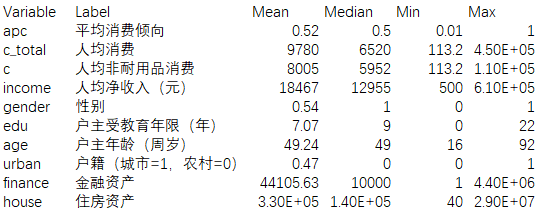
\includegraphics[width=0.8\linewidth]{data_1}
\caption{主要变量的描述性统计(样本容量5812)}
\end{figure}
\end{frame}

\begin{frame}
\frametitle{我国消费异质性程度估计}
\begin{figure}
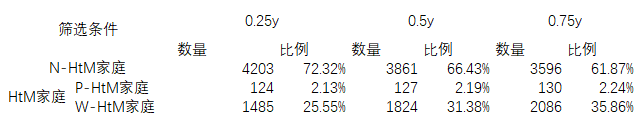
\includegraphics[width=0.8\linewidth]{data_2}
\caption{HtM类家庭与NHtM家庭占比分析(样本容量5812)}
\end{figure}
\end{frame}

\begin{frame}
\frametitle{我国消费异质性程度估计}
\begin{itemize}
\item Kaplan$\&$Violante(2014)利用跨国微观数据估量发现美国、加拿大与德国HtM类型家庭占比约为30$\%$,此数值与本文估量的中国家庭的情况相近
\item 澳大利亚、法国、西班牙、意大利此数值略低于我国,约为20$\%$
\item 各国在P-HtM类型家庭与W-HtM类型家庭的相对数量上存在较大差异,澳大利亚、法国、西班牙此数值与我国接近,意大利P-HtM类型家庭在HtM类型中占比略高于我国,为$7.4\%$,其余国家皆在$10\%$以上
\end{itemize} 
\end{frame}

\section{消费异质性对经济增长路径的影响}

\begin{frame}
\frametitle{消费异质性对经济增长路径的影响}
\begin{itemize}
\item 基于Diamond模型
\item 包含“高流动性,低收益”及“低流动性,高收益”两种资产
\item 假定存在人口组成的更替,一个独立个体在模型中仅存活两期
\item 为简化分析起见,假定时间为离散而非连续的
\item $t=0,1,2$
\item 数量为$L_{t}$的个体在$t$期出生且人口增长率为$n$
\item $L_{t}=(1+n)L_{t-1}$  
\end{itemize}
\end{frame}

\begin{frame}
\frametitle{消费异质性对经济增长路径的影响}
\begin{block}{Block 1}
处于生命周期上半期的每个个体可供给一单位劳动并在该期内做出消费-储蓄决策,在生命的下半周期,个体随着年龄的增长不在劳动,将生命周期上半期的储蓄及资本收入全部用于下半期的消费
\end{block}   

\begin{block}{Block 2}
劳动收入中用于当期收入的部分为“高流动性,低收益”资产而用于储蓄至下半周期并产生资本收入的部分为“低流动性,高收益”资产
\end{block}
\end{frame}

\begin{frame}
\frametitle{消费异质性对经济增长路径的影响}   
分别将生命上半周期及下半周期的消费记为$C_{1,t}$、$C_{2,t+1}$,记出生于$t$的个体整个生命周期内的效用为$U_{t}$

假定效用函数遵循CRRA(constant-relative-risk-aversion)函数形式,设$\rho$个体的主观贴现率,相对风险回避系数为常数$\theta$
\begin{align*}
U_{t}=\frac{C_{1,t}^{1-\theta}-1}{1-\theta}+&\frac{1}{1+\rho}\frac{C_{2,t+1}^{1-\theta}-1}{1-\theta}\\
\theta>0,\qquad & \rho>-1  
\end{align*}
因为下半个生命周期消费的效用贴现后应为正值,个体主观贴现率$\rho$必须大于-1

当$\rho$大于零时,生命周期下半期消费效用的权重$0<\frac{1}{1+\rho}<1$,即个体将更倾向于重视生命周期上半期的效用情况,$\rho$小于零大于-1时则相反

假定模型中有多家完全相同的企业制造产出,每一家企业的生产函数皆为$Y_{t}=F(K_{t},A_{t}L_{t})$,生产函数为规模报酬不变,同时生产函数满足稻田条件
\end{frame}

\begin{frame}
\frametitle{消费异质性对经济增长路径的影响}
每单位有效劳动$AL$对应资本量为$k$,对应产出则为$f(k)=F(k,1)=F(K,AL)/AL$。全要素生产率或配合生产的技术知识$A$保持外生性增长率$g$,即$A_{t}=(1+g)A_{t-1}$

完全竞争,则生产要素资本与劳动都获得其边际产量作为报酬,所有厂商利润为零

参与生产的资本所获得的实际利率为$r_t=f'(k_t)$,每单位有效劳动所获报酬为$w_t=f(k_t)-k_tf'(k_t)$
\end{frame}

\begin{frame}
\frametitle{消费异质性对经济增长路径的影响}
生命周期内消费的预算约束
\begin{equation*}
C_{2,t+1}=(1+r_{t+1})(w_tA_t-C_{1,t})
\end{equation*}
\begin{equation*}
C_{1,t}+\frac{1}{1+r_{t+1}}C_{2,t+1}=A_{t}w_{t}
\end{equation*}
求解个体消费-储蓄决策即求解最优化问题
\begin{align*}
\max U_{t}=\frac{C_{1,t}^{1-\theta}-1}{1-\theta}+&\frac{1}{1+\rho}\frac{C_{2,t+1}^{1-\theta}-1}{1-\theta}\\
s.&t.\\
C_{1,t}+\frac{1}{1+r_{t+1}}C_{2,t+1}&=A_{t}w_{t}
\end{align*}
\end{frame}

\begin{frame}
\frametitle{消费异质性对经济增长路径的影响}
最优化要求
\begin{equation*}
C_{1,t}^{-\theta}\Delta C=\frac{1}{1+\rho}C_{2,t+1}^{-\theta}\Delta C
\end{equation*}
\begin{equation*}
\frac{C_{2,t+1}^\theta}{C_{1,t}^\theta}=\frac{1+r_{t+1}}{1+\rho}
\end{equation*}
\begin{equation*}
\frac{C_{2,t+1}}{C_{1,t}}=\frac{1+r_{t+1}}{1+\rho}^{1/\theta}
\end{equation*}
当资本的实际回报率或实际利率大于主观折现率时,两期而言消费将增加,反之,则下半期消费较上半期减少。$\theta$则决定了个体消费情况对$r$与$\rho$大小变化的反应程度
\end{frame}

\begin{frame}
\frametitle{消费异质性对经济增长路径的影响}
将此欧拉方程代入预算约束可得
\begin{equation*}
C_{1,t}+\frac{(1+r_{t+1})^{(1-\theta)/\theta}}{(1+\rho)^{1/\theta}}C_{1,t}=A_tw_t
\end{equation*}
整理可得
\begin{equation*}
C_{1,t}=\frac{(1+\rho)^{1/\theta}}{(1+\rho)^{1/\theta}+(1+r_{t+1})^{(1-\theta)/\theta}}A_tw_t
\end{equation*}
由于$\rho$与$\theta$皆为常数,则可知生命周期上半期的消费占劳动收入的比例由实际利率决定,储蓄率表示为$s(r_{t+1})=1-C_{1,t}/A_tw_t$
\begin{align*}
s(r)=\frac{(1+r)^{(1-\theta)/\theta}}{(1+\rho)^{1/\theta}+(1+r)^{(1-\theta)/\theta}}\\
C_{1,t}=[1-s(r_{t+1})]A_tw_t
\end{align*}
\end{frame}

\begin{frame}
\frametitle{消费异质性对经济增长路径的影响}   
$s(r)$对于$(1+r)^{(1-\theta)/\theta}$是增函数,可将$(1+r)^{(1-\theta)/\theta}$对实际利率$r$求导可得$[(1-\theta)/\theta](1+r)^{(1-2\theta)/\theta}$,则当$\theta$小于1时,此式对于$r$递增,同样也储蓄率$s$对于$r$递增,相反,当$\theta$大于1时,$s$对于$r$递减。

\vspace{12 pt}

从经济意义上讲,实际利率$r$增加对消费同时具有替代效应和收入效应,当$r$增加时,放弃储蓄在生命周期上半期及时消费的成本变高了。可视为“低流动性,高收益”资产的变现成本更高,因此个体会倾向于在上半期减少消费增加储蓄,而与此同时,同样数额的储蓄将获得更多的资本收入,个体不用大量储蓄收入即可在生命周期下半期充分地享受消费,处于平滑消费的目的,个体会倾向于在上半期增加消费而减少储蓄。当$\theta$较低时,个体对于上下半期消费的替代弹性更高,则此时替代效应起主要作用,而$\theta$较高时,消费的替代弹性较低,个体更愿意在两期内享受相近的消费水平,则收入效应起主要作用。
\end{frame}

\begin{frame}
\frametitle{消费异质性对经济增长路径的影响} 
每一单位有效劳动所获得的资本存量$k$的发展路径
\begin{equation*}
k_{t+1}=\frac{1}{(1+n)(1+g)}s(f'(k_{t+1}))[f(k_t)-k_tf'(k_t)]
\end{equation*}
暂时简单假定$\theta=1$,如前文所述,此时储蓄率$s=1/(2+\rho)$。且假定生产函数满足Cobb-Douglas形式,$f(k)=k^\alpha$则$f'(k)=\alpha k^{\alpha-1}$。
此时$k$的发展路径简化为
\begin{equation*}
k_{t+1}=\frac{1}{(1+n)(1+g)}\frac{1}{2+\rho}(1-\alpha)k_{t}^\alpha
\end{equation*}
\end{frame}

\begin{frame}
\frametitle{消费异质性对经济增长路径的影响}
令$k_{t+1}=k_t=k*$为稳态下的资本存量值,显然当$k*=0$时上式成立,但此种情况由于已假定初始资本存量$K_0$严格大于零而被排除,则由函数形态可判断仅剩一点$k*$可满足
\begin{equation*}
k*=[\frac{1-\alpha}{(1+n)(1+g)(2+\rho)}]^{1/(1-\alpha)}
\end{equation*}
且由于生产函数已知,得到每单位有效劳动的产出
\begin{equation*}
y*=k*^\alpha=[\frac{1-\alpha}{(1+n)(1+g)(2+\rho)}]^{\alpha/(1-\alpha)}
\end{equation*}
\end{frame}

\begin{frame}
\frametitle{消费异质性对经济增长路径的影响}
\section{结论与政策建议}
\begin{itemize}
\item 趋近于均衡发展路径的情况与$\lambda$密切相关
\item 考察不同的冲击或修正对此简易模型中经济均衡发展路径的影响
\item 动态无效率问题
\end{itemize}
\end{frame}

\section{结论与政策建议}
\begin{frame}
\frametitle{结论与政策建议}
\begin{itemize}
\item 削弱国有银行为主体的金融垄断势力,在监管金融风险的同时鼓励金融创新
\item 开发出更多期限不同收益率不同风险特质不同的金融产品以满足居民对于金融多样性的需要
\item 提高金融服务的可得性,开展普惠金融
\item 在政府购买与征税会降低均衡增长路径的资本存量的前提下,应提高政府支出的效益,避免低水平重复建设
\item 完善租房市场,早日实现“租售同权”,对于户籍权益、教育医疗等资源的分配尽量平等
\item 建立运转高效的福利制度,在失业救济、养老、医疗保障方面加大投入以减少不确定性
\end{itemize}
\end{frame}

\begin{frame}
\Huge{\centerline{感谢聆听}}
\end{frame}

\end{document} 